\chapter{Android Application}
\section {Overview}
The application was designed to allow the users to interact with the blockchain. The Application UI was made similar to modern social networks, displaying the nearby events as a scrollable home feed \hyperref[fig:appscreens]{Figure 4.1} shows the different screens design of the Android app.  Authentication is required for the user to login to the blockchain network and to use the app. Once the user successfully authenticated the application will display the nearby events and the app is self-explanatory.

 \begin{figure}[H]
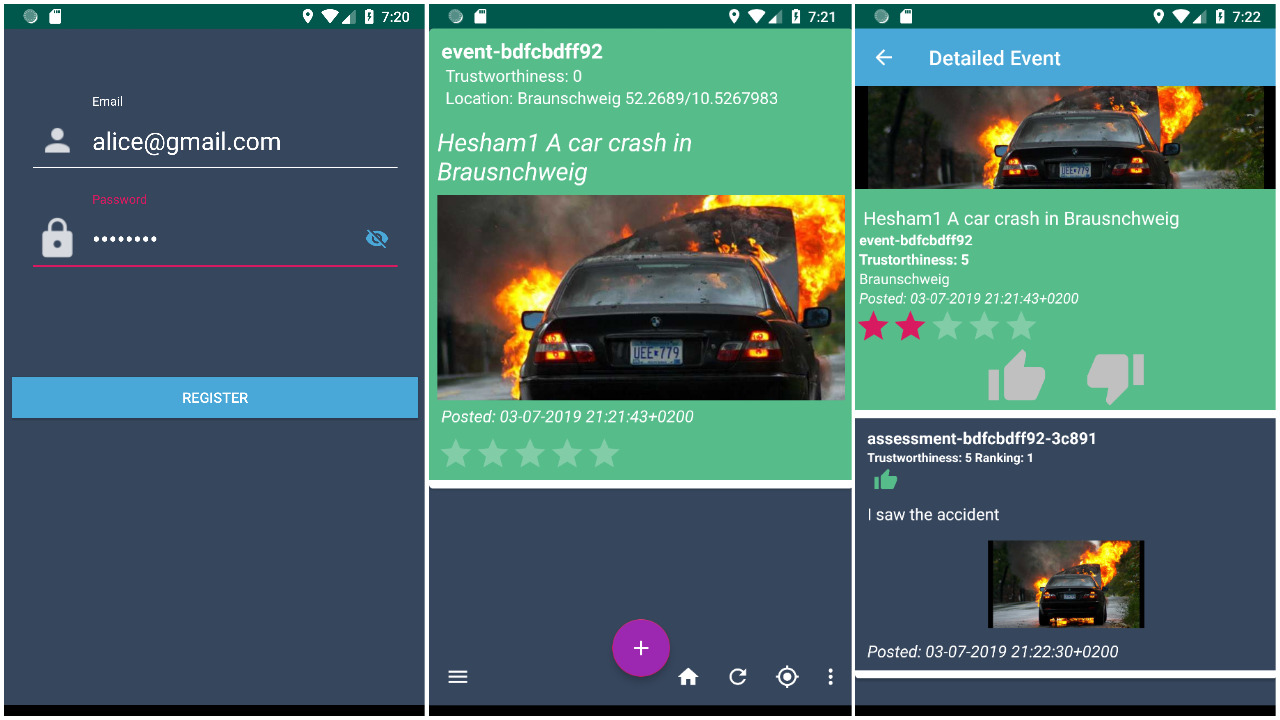
\includegraphics[width=15cm,height=10cm]{images/appscreens.jpg}
\caption{App Screens Represent The Application Design}
\label{fig:appscreens}
\end{figure}
 
\section{The Main Classes} 

In this section, we describe the main classes we used in the application. Every class provided a different functionality.
\subsection{Mainactivity}
MainActiivty is the first activity launched when the application started. it checks if the user logged-in then it will direct the user to registration and login activity. 
Once the user login the email address will be stored in the shared-preference in order to keep the user login. The location access permission will be checked as it's one of the essential parts to continuously fetch the location of the users. A warning message will be displayed to the user if the location access wasn't granted. As long as the location is granted. An enrollment request will be sent using the user's email address as discussed in 3.6 following the enrollment procedures and storing the JWT for making the upcoming requests to the blockchain network.
Finally, the application will use the JWT and the user's location to query the ledger and fetch all the nearby events and displaying them one by one chronologically in the news feed. 
Displaying the feed is nontrivial we used RecyclerView adapter which is an android class used to represent the data dynamically in a separate view and provides the ability to implement both horizontal and vertical layouts. The RecyclerView adapter used to display the data collections whose elements change at runtime based on user action or network events.  In other words every time we query the ledger the user get a JSON response containing all events list. Those events change at run time based on the user's location. The events will be displayed one by one in a separate view similar to Facebook or Instagram posts. 
We created a simple view holder for every event object and we instantiated an object of this view holder and binding the event data to it.    
The same methodology used to display the assessments list.
\hyperref[fig:mainactivityflow]{Figure 4.2} Describes the flow of the Mainactivity. 
 \begin{figure}[H]
\center
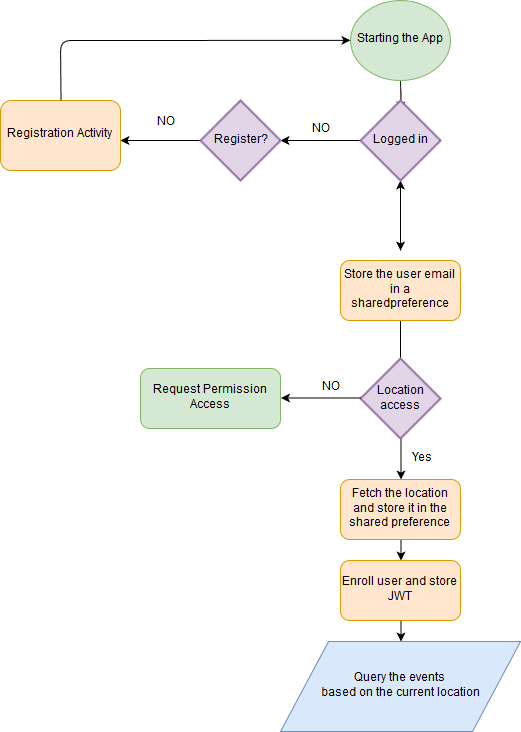
\includegraphics[width=10cm,height=10cm]{images/mainactivityflow.png}
\caption{Mainactivity Flowchart}
\label{fig:mainactivityflow}
\end{figure}

\subsection{AddEvent}
AddEvent is the activity that runs when the user wanted to create a new event. It will prompt the user to upload a photo and an event description. the activity will check the storage's permission access, and if it's granted it will allow the user to select an image from the gallery, then the image will be captured as a bitmap and converted into a string. This string will be hashed and sent to the Xampp server which will rebuild the media file and storing the file with its hash name. In other words, the picture will be stored with its hash and only the hash will be stored on the blockchain for fetching the picture and displaying it directly from the server, not from the blockchain. lastly, the transaction will be invoked by calling addEvent chaincode function name and passing all event's details as parameters.
If the transaction successfully invoked a confirmation message will be displayed to the user that the event is online, Otherwise, an error will be displayed. 
 Storing the hash instead of the entire media file will be more efficient as the file will be replicated many times on the peers.
It's similar to using A CDN which is a standard way to deliver content more quickly and efficiently, based on their geographic location. A content delivery network CDN allows for the quick transfer of assets needed for loading media content including images, and videos. using this approach will increase the performance and decrease the latency. In addition, storing the hash only will save a lot of disk space and assuring that the ledger size will be only a few megabytes instead of hundreds of terabytes. 
   
\hyperref[fig:mainactivityflow]{Figure 4.3} Describes the flow of AddingEvent Activity. 
 \begin{figure}[H]
\center
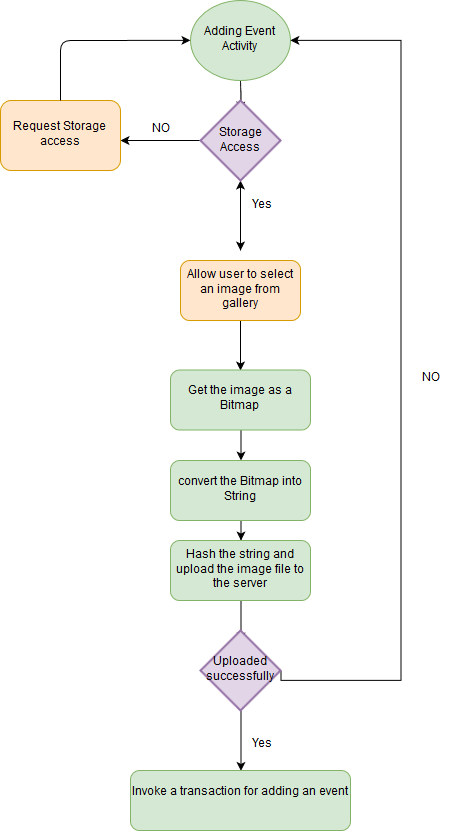
\includegraphics[width=8cm,height=12cm]{images/addingeventflowchart.png}
\caption{Addevent Flowchart}
\label{fig:addingeventflowchart}
\end{figure}

\cleardoublepage

\subsection{The Hashing Method}
For a more efficient way of storing data on the blockchain, only the media file is hashed and only the hash of it will be stored on CDN like S3 we store the data on a simple Xampp server for development purpose. the media file will be easily fetched and displayed. 
\textbf{PBKDF2} Algorithm is implemented. this hash function is slow enough to impede attacks, but still fast enough to not cause a noticeable delay for the users. A simple implementation of the hashing algorithm in listing 4.1.

 \begin{lstlisting}[caption={PBKDF2 Simple Implementation},captionpos=b]
import javax.crypto.SecretKeyFactory;
import javax.crypto.spec.PBEKeySpec;
import java.math.BigInteger;

public class Hashing {

    private static final int ITERATIONS = 1000;
    private static final int KEY_LENGTH = 192; // bits
    public static final String SALT = "Random Salt" ;

    public static String hashPassword(String password, String salt){
        char[] passwordChars = password.toCharArray();
        byte[] saltBytes = salt.getBytes();
        PBEKeySpec spec = new PBEKeySpec(
                passwordChars,
                saltBytes,
                ITERATIONS,
                KEY_LENGTH
        );
        SecretKeyFactory key = null;
        try {
            key = SecretKeyFactory.getInstance("PBKDF2WithHmacSHA1");
        } catch (NoSuchAlgorithmException e) {
            e.printStackTrace();
        }
        byte[] hashedPassword = new byte[0];
        try {
            hashedPassword = key.generateSecret(spec).getEncoded();
        } catch (InvalidKeySpecException e) {
            e.printStackTrace();
        }
        return String.format("%x", new BigInteger(hashedPassword));
    }
}
\end{lstlisting}
\cleardoublepage


\subsection{Voting}
When the user selects on a specific event a new activity will be created, and the event will be separately displayed with more details about the event, and the application will allow the user to judge or assess the event by up-voting or down-voting, also it would be possible to attach a description or a media file.
The voting activity is similar to adding an event the data will be stored captured media file will be hashed and uploaded to the server and finally, a transaction will be invoked and judgeEvent chaincode function will be invoked and all assessments details will be passed as parameters. in the end, a confirmation message will be displayed in case of success and an error in case of any failure or network error. 
Assessing events will credit or discredit a specific event and directly reflects the creator of the event's reputation score. 
The voting is similar to adding the event activity just different in calling the judgeEvent. 


\subsection{Login and Register}
In order to allow the users to log-in and register, we implemented two separate activities. the user will input an email and password, then we are validating the user input. and an error will be displayed if the email address is not valid or empty or in use by another user. 
If the data was valid we submit a request over the network and store it to the relational database. The email will be stored in a plain text, however, the password will be stored hashed. 
Similarly, the login activity once the user inputs his email and password it will be checked against the database if the credentials were correct the access is granted to the user and the email will be saved to keep the user logged in.

\cleardoublepage

\subsection{Ranking and Trustworithness} 

One of the main features we introduced is ranking the events and calculating users' reputation.
The user's reputation will depend on the user's interaction on the platform. how frequent he participated, how many good reviews he received on the event he created. 
Every user starts with 0 reputation score. Adding an event will increase his score by +1.  \\
The algorithm considers the users rank and location's trustworthiness or how close is the user from the event.
Assume a user with score 510 and was about 10 meters away from an event he is going to assess. First, we convert the score into stars as the user's reputation score is 510 then the stars function will return 5. Second, we calculate how far is the user and return a value from 1 (almost in the scene of the event he is assessing)  to .1 (so far away from the event) in this case the closeness function will emit 1 so the final score the user is 25. This score will increase/decrease in the assessed event's trustworthiness. Depending on the vote type if it's up/down vote this will credit or discredit the event's trustworthiness and increase or decrease the overall reputation score of the event creator. 
Once the assessment is made the chaincode updates the assessed event's trustworthiness and the event creator's reputation score.
In summary, What easily influences the user’s reputation and the event's trustworthiness is getting good/bad reviews from the highly ranked users who are very nearby to the assessed event. 
\hyperref[fig:mainactivityflow]{Figure 4.4} describes the ranking algorithm. 
 \begin{figure}[H]
\center
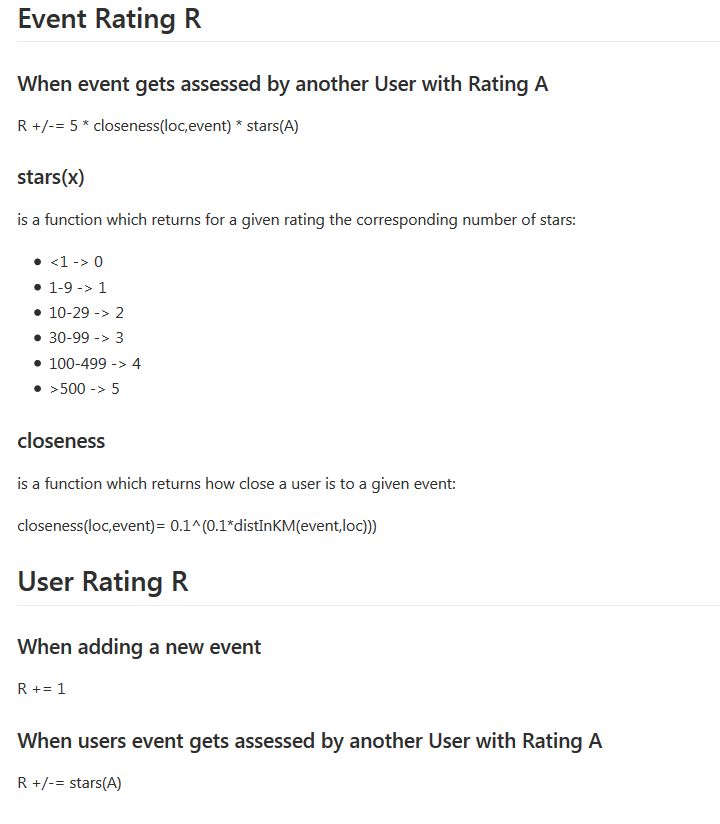
\includegraphics[width=14cm,height=13cm]{images/ranking.png}
\caption{The Ranking Algorithm}
\label{fig:ranking}
\end{figure}
 